% Sjálfstætt Overleaf-skjal. Veljið pdfLaTeX. UTF-8.
% Allur stíll og allar TikZ-myndir eru í þessari skrá.
\documentclass[12pt,letterpaper]{article}
\usepackage[T1]{fontenc}
\usepackage[utf8]{inputenc}
\usepackage[icelandic]{babel}
\usepackage{lmodern,amsmath,amssymb}
\usepackage[margin=20mm,headheight=15pt]{geometry}
\usepackage{xcolor,tikz}
\usetikzlibrary{arrows.meta,calc,angles,quotes}
\usepackage[most]{tcolorbox}
\usepackage{array,tabularx,longtable,booktabs,enumitem,needspace,microtype}
\usepackage{hyperref}
\definecolor{lotaBlue}{HTML}{0877C9}
\definecolor{lotaGreen}{HTML}{24C95A}
\definecolor{lotaCyan}{HTML}{54C8F2}
\definecolor{lotaMagenta}{HTML}{D962CF}
\definecolor{lotaYellow}{HTML}{FFD966}
\definecolor{lotaPalePink}{HTML}{F3CBEF}
\definecolor{lotaStep}{HTML}{F4A261}
\hypersetup{colorlinks=true,linkcolor=lotaBlue,urlcolor=lotaBlue,
pdftitle={Lota 29: Rúmmál og yfirborð},pdfauthor={Námsefni fyrir 10. bekk}}
\setlength{\parindent}{0pt}
\setlength{\parskip}{6pt}
\setlength{\emergencystretch}{2em}
\setlist[itemize]{nosep,leftmargin=1.5em}
\setlist[enumerate]{itemsep=3pt,topsep=3pt,leftmargin=1.8em}
\newcommand{\timi}[2]{\clearpage\phantomsection\label{timi:lota29-0#1}
\begin{center}{\large\bfseries Lota 29: #1. tími}\par\medskip
{\fontsize{20}{24}\selectfont\bfseries #2}\end{center}}
\newcommand{\kafli}[1]{\par\Needspace{5\baselineskip}{\large\bfseries #1}\par}
\newcommand{\hugtak}[2]{\hyperref[hugtak:#1]{\textbf{#2}}}
\newcommand{\skref}[1]{\par\smallskip\colorbox{lotaStep}{\strut\textbf{SKREF #1}}\quad}
\newenvironment{daemi}[2][lotaGreen]{\par\Needspace{7\baselineskip}
\noindent\colorbox{#1}{\strut\textbf{DÆMI}}\quad\textbf{#2}\par\nopagebreak
\begin{tcolorbox}[enhanced,breakable,colback=white,colframe=#1!35!white,
boxrule=.7pt,sharp corners,left=8pt,right=8pt,top=6pt,bottom=6pt]}{\end{tcolorbox}}
\newtcolorbox{regla}{colback=lotaYellow,colframe=black!45,boxrule=.4pt,sharp corners,breakable}
\newtcolorbox{mundu}{colback=lotaPalePink,colframe=black!45,boxrule=.4pt,sharp corners,breakable}
\newcommand{\markmid}[1]{\textbf{Þetta lærir þú:} #1\par}
\newcommand{\gloss}[4]{\par\Needspace{4\baselineskip}\phantomsection\label{hugtak:#1}
\textbf{#2.} #3\quad\hyperref[timi:lota29-0#4]{Sjá #4. tíma, bls.\ \pageref*{timi:lota29-0#4}.}\par}
\newcommand{\gat}[1]{\par\noindent\(\square\)\quad #1\par}
\tikzset{every picture/.style={line width=.8pt},>=Stealth}

\newcommand{\eining}[1]{\,\mathrm{#1}}
\newcommand{\myndtexti}[1]{{\small #1}\par}
\newcommand{\nyrhluti}[1]{\newpage\kafli{#1}}
\newcommand{\tolur}[1]{{\color{lotaBlue}#1}}
\newcommand{\yfirlitslina}[3]{\hyperref[timi:lota29-0#1]{#1}&\hyperref[timi:lota29-0#1]{\textbf{#2}} #3&\pageref{timi:lota29-0#1}\\}
\newcommand{\teningsmynd}{%
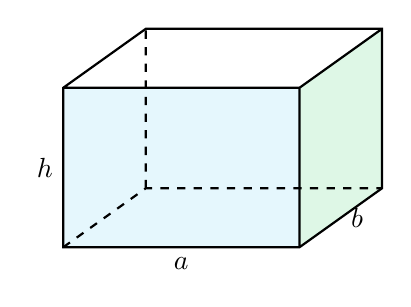
\begin{tikzpicture}[scale=.75]
\coordinate (A) at (0,0);\coordinate (B) at (4,0);\coordinate (C) at (5.4,1);\coordinate (D) at (1.4,1);
\coordinate (E) at (0,2.7);\coordinate (F) at (4,2.7);\coordinate (G) at (5.4,3.7);\coordinate (H) at (1.4,3.7);
\fill[lotaCyan!15] (A)--(B)--(F)--(E)--cycle;\fill[lotaGreen!15] (B)--(C)--(G)--(F)--cycle;
\draw (A)--(B)--(C)--(G)--(H)--(E)--cycle (E)--(F)--(G) (B)--(F);
\draw[dashed] (A)--(D)--(C) (D)--(H);
\node[below] at (2,0){$a$};\node[right] at (4.7,.5){$b$};\node[left] at (0,1.35){$h$};
\end{tikzpicture}}


\begin{document}
\begin{center}
{\large\bfseries Lota 29 · 10. bekkur}\par\bigskip
{\fontsize{22}{27}\selectfont\bfseries RÚMMÁL OG YFIRBORÐ}\par\medskip
{\large Lesefni fyrir sjö kennslutíma}
\end{center}
\phantomsection\label{yfirlit}
\kafli{Yfirlit}
Hversu mikið rúmast í íláti? Hve mikið efni þarf utan um hlut? Í þessari lotu tengjum við myndir, einingar og formúlur. Ný sýnidæmi sýna aðferðir sem þú getur síðan notað sjálf eða sjálfur í verkefnunum.
\renewcommand{\arraystretch}{1.4}
\begin{tabularx}{\linewidth}{@{}c X r@{}}
\toprule\textbf{Tími}&\textbf{Viðfangsefni}&\textbf{Bls.}\\\midrule
\yfirlitslina{1}{Ferstrendingar.}{Rúmmál, lítrar, yfirborð, massi og stærðarbreytingar.}
\yfirlitslina{2}{Strendingar.}{Grunnflötur, möttull, samsett þversnið og hallandi botn.}
\yfirlitslina{3}{Sívalningar.}{Hringflötur, rúmmál, umbúðir og efnisnotkun.}
\yfirlitslina{4}{Strýtur.}{Pýramídar, keilur, skáhlið og samsett rúmmál.}
\yfirlitslina{5}{Kúlur.}{Rúmmál og yfirborð kúlu og hálfkúlu, endurmótun og massi.}
\yfirlitslina{6}{Hagnýt dæmi I.}{Val á formúlu, samsettir hlutir, óþekkt hæð og prósentur.}
\yfirlitslina{7}{Hagnýt dæmi II.}{Hlutföll, óþekktar lengdir, Pýþagóras og ytra yfirborð.}
\bottomrule
\end{tabularx}
\medskip
\hyperref[gatlisti]{Gátlisti} er á bls.\ \pageref{gatlisti} og \hyperref[hugtok]{hugtök lotunnar} á bls.\ \pageref{hugtok}.
\begin{mundu}\textbf{Svona nýtir þú heftið:} Lestu skýringuna og myndina saman. Reyndu næsta skref áður en þú lest áfram. Blá hugtök eru smellanleg og leiða að skilgreiningum aftast.\end{mundu}
\kafli{Tákn sem fylgja okkur}
\(R\): rúmmál, \(G\): grunnflatarmál, \(Y\): yfirborðsflatarmál, \(M\): flatarmál möttuls, \(U\): ummál grunnflatar. Lengdir eru skilgreindar við hverja mynd.

\timi{1}{FERSTRENDINGAR}
\markmid{Að reikna rúmmál og yfirborð kassa, breyta einingum, finna massa og bera saman misstóra kassa.}
\kafli{Rúmmál er fjöldi rúmeininga}
\hugtak{ferstrendingur}{Rétthyrndur ferstrendingur} hefur sex rétthyrnda fleti. Hér köllum við hann ferstrending eða kassa. \hugtak{rummal}{Rúmmál} segir hve mikið rými hlutur tekur eða hve mikið rúmast innan í honum.
\begin{center}\teningsmynd\par\myndtexti{Skýringarmynd í rúmsýn; $a$ og $b$ eru grunnbrúnir og $h$ er hæð.}\end{center}
Á botninum rúmast \(a\cdot b\) einingar í hverju lagi og lögin eru \(h\). Þess vegna er \(R=abh\).
\begin{regla}\textbf{FLÝTILEIÐ: Einingar}\par
\(1\eining{dm^3}=1\eining{\ell}\), \quad \(1000\eining{cm^3}=1\eining{\ell}\), \quad \(1\eining{m^3}=1000\eining{\ell}\).\par
\(1\eining{cm^3}=1\eining{m\ell}\), \quad \(1\eining{c\ell}=10\eining{cm^3}\).\par
Þegar lengdareining breytist tífalt breytist flatarmálseining hundraðfalt og rúmmálseining þúsundfalt.
\end{regla}
\begin{daemi}{1.1 · Rúmmál geymslukassa}
Innanmál kassa fyrir föndurefni eru \(48\times25\times32\) cm.
\[\tolur{R=48\cdot25\cdot32=38400\eining{cm^3}=38{,}4\eining{\ell}.}\]
Annar kassi hefur innanmálin \(620\times450\times800\) mm. Í dm eru þau \(6{,}2\times4{,}5\times8\), svo
\[R=6{,}2\cdot4{,}5\cdot8=223{,}2\eining{dm^3}=223{,}2\eining{\ell}.\]
\end{daemi}
\begin{mundu}\textbf{MUNDU:} Notaðu sömu lengdareiningu í öllum þáttum. Innanmál gefa rúmmál. Utanmál innihalda líka efnisþykkt kassans.\end{mundu}

\nyrhluti{Yfirborð: leggja saman réttu fletina}
\hugtak{yfirbord}{Yfirborðsflatarmál} er samanlagt flatarmál ytri flata. Lokaður kassi hefur tvö eintök af hverjum fleti: \(ab\), \(ah\) og \(bh\).
\begin{regla}\textbf{FLÝTILEIÐ:} Lokaður ferstrendingur: \(Y=2ab+2ah+2bh\).\par
Opinn kassi án loks: \(Y=ab+2ah+2bh\). Þetta gildir þegar botninn er \(a\times b\).\end{regla}
\begin{daemi}[lotaCyan]{1.2 · Efni í lokaðan kassa}
Mál líkankassa eru \(4{,}2\) cm, \(3{,}1\) cm og \(2{,}6\) cm.
\[Y=2(4{,}2\cdot3{,}1+4{,}2\cdot2{,}6+3{,}1\cdot2{,}6)=64\eining{cm^2}.\]
Í stærri verkfærakassa eru málin \(640\times300\times280\) mm, eða \(0{,}64\times0{,}30\times0{,}28\) m. Þá þarf að lágmarki
\[Y=2(0{,}192+0{,}1792+0{,}084)=0{,}9104\eining{m^2}\]
af plötuefni. Hér er gert ráð fyrir loki, engri skörun og engu afskurðartapi. Tveir slíkir kassar þurfa tvöfalt þetta flatarmál.
\end{daemi}
\kafli{Teningur og snið}
\hugtak{teningur}{Teningur} hefur sex eins ferningsfleti. \hugtak{net}{Snið} sýnir fletina útbreidda í sléttum fleti.
\begin{center}
\begin{tikzpicture}[scale=.62]
\foreach \x/\y in {0/0,1.5/0,3/0,4.5/0,1.5/1.5,1.5/-1.5}{\draw[fill=lotaCyan!16] (\x,\y) rectangle ++(1.5,1.5);}
\node[above] at (2.25,3){$s=3{,}5$ cm};
\node[right,align=left] at (6.7,.8){Sex ferningar\\verða sex fletir.};
\end{tikzpicture}
\end{center}
\begin{daemi}[lotaMagenta]{1.3 · Frá sniði að rúmmáli}
Hver brún er \(s=3{,}5\) cm. Því er
\[R=s^3=42{,}875\eining{cm^3},\qquad Y=6s^2=73{,}5\eining{cm^2}.\]
Rúmmál og yfirborðsflatarmál svara ólíkum spurningum og hafa ólíkar einingar.
\end{daemi}

\nyrhluti{Frá rúmmáli að massa eða magni}
\hugtak{edlismassi}{Eðlismassi} segir til um massa hverrar rúmeiningar. Ef hver rúmsentímetri vegur \(\rho\) grömm er massinn \(m=\rho R\), þar sem \(R\) er í cm\(^3\).
\begin{daemi}{1.4 · Massi steinblokkar}
Steinblokk er \(12\times7\times4\) cm. Gefið er að hver cm\(^3\) vegi \(2{,}5\) g.
\[R=12\cdot7\cdot4=336\eining{cm^3},\qquad m=2{,}5\cdot336=840\eining{g}.\]
Svarið er \(0{,}84\) kg. Rúmmálseiningarnar verða að passa við einingarnar í gefnum eðlismassa.
\end{daemi}
\begin{daemi}[lotaCyan]{1.5 · Hlutfallslegt magn í líkani}
Í reiknilíkani er rétthyrndur vatnsgeymir \(18\) m langur, \(7\) m breiður og \(1{,}6\) m djúpur. Í litunartilraun er gert ráð fyrir einum lítra af litlausn á hverja \(24\eining{m^3}\).
\[R=18\cdot7\cdot1{,}6=201{,}6\eining{m^3}.\]
Fjöldi \(24\eining{m^3}\) skammta er \(201{,}6/24=8{,}4\). Því þarf \(8{,}4\) lítra af lausn í þessu líkani.
\end{daemi}
\kafli{Allar lengdir breytast í sama hlutfalli}
Ef allar lengdir margfaldast með \hugtak{staerdarhlutfall}{stærðarhlutfallinu} \(k>0\), margfaldast flatarmál með \(k^2\) og rúmmál með \(k^3\). Ástæðan sést í \((ka)(kb)=k^2ab\) og \((ka)(kb)(kh)=k^3abh\).
\begin{daemi}[lotaMagenta]{1.6 · Litlir gjafakassar og efniskostnaður}
Stór kassi er \(18\times12\times9\) cm. Allar brúnir litla kassans eru þriðjungur af samsvarandi stórum brúnum.
\[R_{\text{stór}}=1944\eining{cm^3}=1{,}944\eining{\ell},\qquad
R_{\text{lítill}}=\frac{1944}{27}=72\eining{cm^3}.\]
Það þarf \(27\) litla kassa fyrir sama rúmmál. Efnismagn í einn lítinn kassa er hins vegar \(1/9\) af efnismagni í stóran; sama efni dugar í \(9\) litla kassa ef ekkert fer til spillis.

Ef efnið í stóran kassa kostar \(630\) kr. og kostnaður er í réttu hlutfalli við flatarmál, kostar efnið í lítinn \(630/9=70\) kr. Efnið í \(27\) litla kostar \(1890\) kr.
\end{daemi}

\timi{2}{STRENDINGAR}
\markmid{Að velja grunnflöt, reikna rúmmál og möttul og skipta samsettu formi í einfaldari hluta.}
\kafli{Sami grunnflötur alla leið}
\hugtak{strendingur}{Strendingur} hefur tvo eins og samsíða marghyrnda grunnfleti. Í réttum strendingi standa hliðarbrúnir hornrétt á grunnfletina. Við vinnum með rétta strendinga hér.

\hugtak{grunnflotur}{Grunnflötur} þarf ekki að vera neðsti flöturinn á mynd. Í liggjandi þrístrendingi getum við valið þríhyrningana á endunum sem grunnfleti. \hugtak{haed}{Hæð strendingsins} er hornrétta fjarlægðin milli grunnflatanna, oft kölluð lengd þegar hluturinn liggur.
\begin{regla}\textbf{FLÝTILEIÐ:} Fyrir strending er \(R=G h\).\par
Finndu fyrst grunnflatarmálið \(G\), síðan fjarlægðina \(h\) milli grunnflatanna. Fyrir þríhyrning er \(G=bg/2\), þar sem \(g\) er hornrétt hæð á grunnlínuna \(b\).\end{regla}
\begin{center}
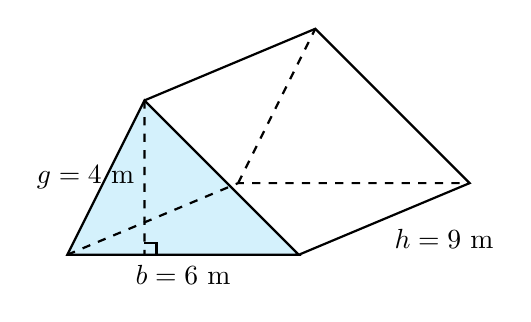
\begin{tikzpicture}[scale=.7]
\coordinate (A) at (0,0);\coordinate (B) at (4.2,0);\coordinate (C) at (1.4,2.8);
\fill[lotaCyan!25] (A)--(B)--(C)--cycle;
\draw (A)--(B)--(C)--cycle (B)--node[midway,below right]{$h=9$ m}(7.3,1.3)--(4.5,4.1)--(C);
\draw[dashed] (A)--(3.1,1.3)--(7.3,1.3) (3.1,1.3)--(4.5,4.1);
\draw[dashed] (C)--node[left]{$g=4$ m}(1.4,0);\draw (1.4,.22)--(1.62,.22)--(1.62,0);
\node[below] at (2.1,0){$b=6$ m};
\end{tikzpicture}\par\myndtexti{Skýringarmynd, ekki í kvarða. $g$ og $h$ eru ólíkar hæðir.}
\end{center}
\begin{daemi}{2.1 · Þríhyrndur grunnflötur}
\[G=\frac{6\cdot4}{2}=12\eining{m^2},\qquad R=12\cdot9=108\eining{m^3}.\]
Hæð þríhyrningsins kemur við sögu þegar \(G\) er fundið. Hæð strendingsins kemur við sögu þegar margfaldað er með fjarlægðinni milli endanna.
\end{daemi}
\begin{daemi}[lotaCyan]{2.2 · Grunnflatarmálið er þegar gefið}
Strendingur er \(18\) cm á hæð. Ef \(G=46\eining{cm^2}\) er \(R=46\cdot18=828\eining{cm^3}\). Ef \(G=73\eining{cm^2}\) er \(R=1314\eining{cm^3}\). Ekki reikna grunnflatarmálið aftur eða deila því með tveimur.
\end{daemi}

\nyrhluti{Möttull og lokaður þrístrendingur}
\hugtak{mottull}{Möttull} er safn hliðarflatanna, án grunnflatanna tveggja. Þegar möttull rétts strendings er breiddur út fást rétthyrningar með sameiginlega hæð \(h\). Breiddir þeirra leggjast saman í \hugtak{ummal}{ummál} grunnflatarins, \(U\).
\begin{regla}\textbf{FLÝTILEIÐ:} Réttur strendingur: \(M=Uh\).\par
Lokaður strendingur: \(Y=M+2G\). Fyrir rúmmál þarftu \(G\); fyrir möttul þarftu \(U\).\end{regla}
\begin{daemi}[lotaMagenta]{2.3 · Rétthyrndur þríhyrningur á endunum}
Grunnflötur hlutar hefur skammhliðar \(1{,}5\) m og \(2{,}0\) m. Lengd strendingsins er \(3{,}2\) m.
\skref{1} Grunnflatarmál og rúmmál:
\[G=\frac{1{,}5\cdot2}{2}=1{,}5\eining{m^2},\qquad
R=1{,}5\cdot3{,}2=4{,}8\eining{m^3}=4800\eining{\ell}.\]
\skref{2} Finndu þriðju hlið þríhyrningsins með \hugtak{pythagoras}{Pýþagórasarreglu}:
\[c=\sqrt{1{,}5^2+2^2}=2{,}5\eining{m}.\]
\skref{3} Möttull og heildaryfirborð:
\[U=1{,}5+2+2{,}5=6\eining{m},\qquad M=6\cdot3{,}2=19{,}2\eining{m^2}.\]
\[Y=19{,}2+2\cdot1{,}5=22{,}2\eining{m^2}.\]
\end{daemi}
\begin{center}
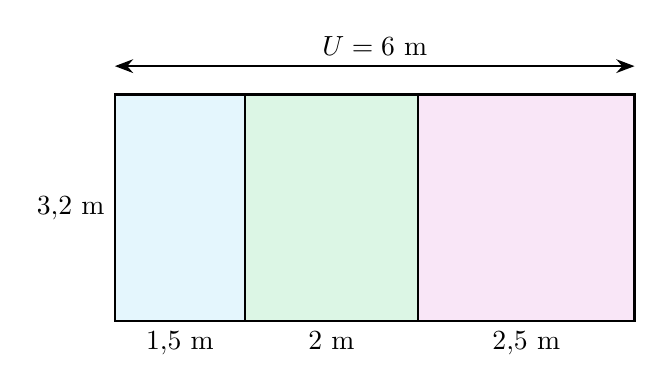
\begin{tikzpicture}[x=1.1cm,y=.9cm]
\draw[fill=lotaCyan!16] (0,0) rectangle (1.5,3.2);
\draw[fill=lotaGreen!16] (1.5,0) rectangle (3.5,3.2);
\draw[fill=lotaMagenta!16] (3.5,0) rectangle (6,3.2);
\node[below] at (.75,0){$1{,}5$ m};\node[below] at (2.5,0){$2$ m};\node[below] at (4.75,0){$2{,}5$ m};
\node[left] at (0,1.6){$3{,}2$ m};\draw[<->] (0,3.6)--node[above]{$U=6$ m}(6,3.6);
\end{tikzpicture}\par\myndtexti{Möttullinn útbreiddur: þrír rétthyrningar. Endafletirnir eru ekki sýndir.}
\end{center}
\begin{mundu}\textbf{MUNDU:} Það að hlutur sé lokaður í báða enda bætir tveimur grunnflötum við yfirborðið. Rúmmálsformúlan breytist ekki.\end{mundu}

\nyrhluti{Samsett þversnið}
\hugtak{thversnid}{Þversnið} er flöturinn sem kemur í ljós þegar skorið er þvert í gegnum hlut. Sé sama þversnið alla leið má nota það sem grunnflöt strendings.
\begin{daemi}{2.4 · Tvö þrep}
Steyptur pallur hefur þversniðið á myndinni og er \(1{,}10\) m breiður. Bæði þrep eru \(0{,}18\) m há; efri flöturinn er \(0{,}42\) m langur og sá neðri nær \(0{,}28\) m lengra fram.
\begin{center}
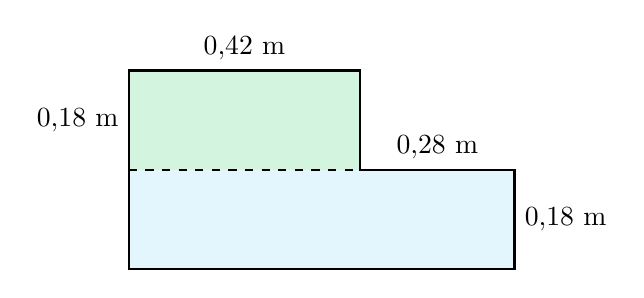
\begin{tikzpicture}[x=7cm,y=7cm]
\fill[lotaCyan!16] (0,0) rectangle (.7,.18);
\fill[lotaGreen!20] (0,.18) rectangle (.42,.36);
\draw (0,0)--(.7,0)--(.7,.18)--(.42,.18)--(.42,.36)--(0,.36)--cycle;
\draw[dashed] (0,.18)--(.42,.18);
\node[above] at (.21,.36){$0{,}42$ m};\node[above] at (.56,.18){$0{,}28$ m};
\node[right] at (.7,.09){$0{,}18$ m};\node[left] at (0,.27){$0{,}18$ m};
\end{tikzpicture}
\end{center}
Neðri rétthyrningurinn er \(0{,}70\) m langur. Því er
\[G=0{,}70\cdot0{,}18+0{,}42\cdot0{,}18=0{,}2016\eining{m^2},\]
\[R=0{,}2016\cdot1{,}10=0{,}22176\eining{m^3}.\]
Hlutarnir skarast ekki; hvert steinsteypukorn er talið einu sinni.
\end{daemi}
\begin{daemi}[lotaCyan]{2.5 · Trapisa í þversniði}
Rás er \(14\) m löng. Þversniðið er \hugtak{trapisa}{trapisa} með samsíða hliðar \(1{,}8\) m og \(0{,}8\) m og hornrétta hæð \(1{,}1\) m.
\[G=\frac{1{,}8+0{,}8}{2}\cdot1{,}1=1{,}43\eining{m^2},\qquad R=20{,}02\eining{m^3}.\]
Formúlan notar meðaltal breiddanna margfaldað með dýptinni.
\end{daemi}
\begin{daemi}[lotaMagenta]{2.6 · Hús með risþaki}
Geymsluhús er \(14\) m langt og \(8\) m breitt. Veggir eru \(3\) m háir og mænir \(5{,}5\) m yfir gólfi. Þakhæðin ofan við veggi er því \(2{,}5\) m.
\[G=8\cdot3+\frac{8\cdot2{,}5}{2}=34\eining{m^2},\qquad R=34\cdot14=476\eining{m^3}.\]
Hér er framhliðin rétthyrningur og þríhyrningur saman.
\end{daemi}

\nyrhluti{Hallandi botn: rúmmál, botn og veggir}
\begin{daemi}[lotaCyan]{2.7 · Laug með þremur botnhlutum}
Æfingalaug er \(20\) m löng og \(9\) m breið. Dýptin er \(0{,}9\) m í grunna endanum og \(2{,}4\) m í þeim djúpa. Botninn er láréttur fyrstu \(4\) m, hallar næstu \(10\) m \textbf{mælt lárétt} og er láréttur síðustu \(6\) m.
\begin{center}
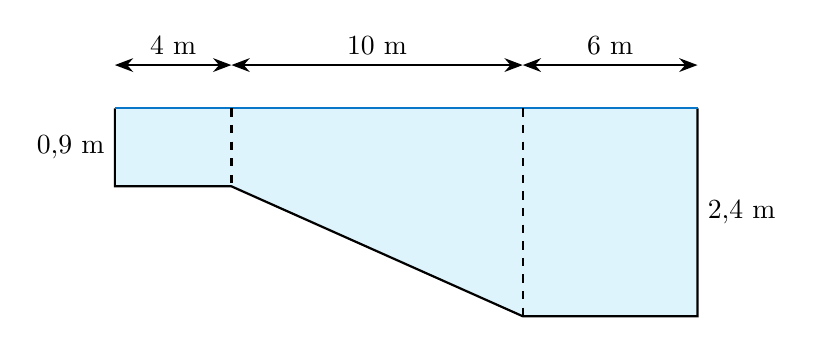
\begin{tikzpicture}[x=.37cm,y=1.1cm]
\fill[lotaCyan!20] (0,0)--(20,0)--(20,-2.4)--(14,-2.4)--(4,-.9)--(0,-.9)--cycle;
\draw[thick] (0,0)--(0,-.9)--(4,-.9)--(14,-2.4)--(20,-2.4)--(20,0);
\draw[lotaBlue] (0,0)--(20,0);
\draw[dashed] (4,0)--(4,-.9) (14,0)--(14,-2.4);
\draw[<->] (0,.5)--node[above]{4 m}(4,.5);
\draw[<->] (4,.5)--node[above]{10 m}(14,.5);
\draw[<->] (14,.5)--node[above]{6 m}(20,.5);
\node[left] at (0,-.45){$0{,}9$ m};\node[right] at (20,-1.2){$2{,}4$ m};
\end{tikzpicture}\par\myndtexti{Langsnið. Lóðréttur og láréttur kvarði eru ólíkir svo hallinn sjáist skýrt.}
\end{center}
\skref{1} Flatarmál langsniðsins er tveir rétthyrningar og trapisa:
\[G=4\cdot0{,}9+10\cdot\frac{0{,}9+2{,}4}{2}+6\cdot2{,}4=34{,}5\eining{m^2}.\]
Rúmmálið fæst með því að margfalda með breiddinni:
\[\tolur{R=34{,}5\cdot9=310{,}5\eining{m^3}.}\]
\skref{2} Flísar á botni fylgja hallanum. Hæðarmunurinn er \(1{,}5\) m og raunveruleg lengd hallans er
\[s=\sqrt{10^2+1{,}5^2}=\sqrt{102{,}25}\eining{m}.\]
Botnflatarmálið er því
\[F_{\text{botn}}=9(4+\sqrt{102{,}25}+6)\approx181{,}01\eining{m^2}.\]
\skref{3} Langveggirnir eru tveir, hvor eins og langsniðið. Endaveggirnir eru rétthyrningar:
\[F_{\text{veggir}}=2\cdot34{,}5+9\cdot0{,}9+9\cdot2{,}4=98{,}7\eining{m^2}.\]
\end{daemi}
\begin{mundu}\textbf{ATH.:} Lárétt lengd hallakafla og lengd eftir hallanum eru ólíkar. Ef lengdin eftir hallanum er gefin, finnst lárétta lengdin með \(x=\sqrt{s^2-(\Delta h)^2}\). Skráðu alltaf hvaða lengd er gefin.\end{mundu}

\timi{3}{SÍVALNINGAR}
\markmid{Að reikna rúmmál sívalnings, greina radíus frá þvermáli og finna efni í möttul.}
\kafli{Hringflötur alla leið}
Réttur \hugtak{sivalningur}{sívalningur} hefur tvo eins hringlaga grunnfleti. Fjarlægðin milli þeirra er hæðin \(h\), líka þegar sívalningurinn liggur. \hugtak{radius}{Radíus} \(r\) er fjarlægðin frá miðju hrings að jaðri. \hugtak{thvermal}{Þvermál} \(\text{\th}\) liggur þvert yfir miðjuna: \(\text{\th}=2r\).
\begin{center}
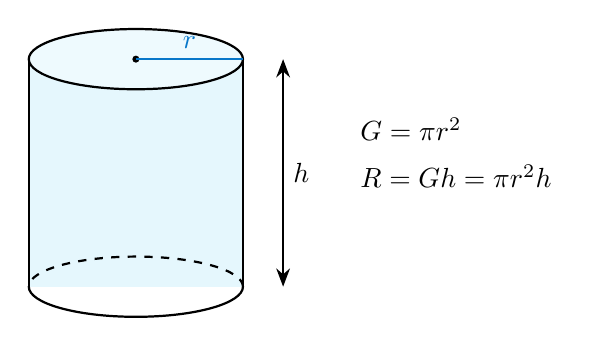
\begin{tikzpicture}[scale=.85]
\fill[lotaCyan!15] (-1.6,0) rectangle (1.6,3.4);
\draw (-1.6,0)--(-1.6,3.4) (1.6,0)--(1.6,3.4);
\draw[fill=lotaCyan!10] (0,3.4) ellipse (1.6 and .45);
\draw (1.6,0) arc[start angle=0,end angle=-180,x radius=1.6,y radius=.45];
\draw[dashed] (1.6,0) arc[start angle=0,end angle=180,x radius=1.6,y radius=.45];
\fill (0,3.4) circle(1.5pt);\draw[lotaBlue,thick] (0,3.4)--node[above]{$r$}(1.6,3.4);
\draw[<->] (2.2,0)--node[right]{$h$}(2.2,3.4);
\node[align=left,right] at (3.2,2){$G=\pi r^2$\\[5pt]$R=Gh=\pi r^2h$};
\end{tikzpicture}\par\myndtexti{Skýringarmynd í rúmsýn. Hringfletir birtast sem sporbaugar á teikningunni.}
\end{center}
\begin{regla}\textbf{FLÝTILEIÐ:} \(R=\pi r^2h\). Ef þvermál er gefið skaltu fyrst reikna \(r=\frac{\text{\th}}{2}\). Notaðu \(\pi\)-takkann og námundaðu lokasvarið.\end{regla}
\begin{daemi}{3.1 · Sívalningslaga ílát}
Innanradíus íláts er \(4{,}5\) cm og hæð þess \(18\) cm.
\[R=\pi\cdot4{,}5^2\cdot18=364{,}5\pi\eining{cm^3}\approx1145{,}11\eining{cm^3}.\]
Ílátið rúmar um \(1{,}15\) lítra. Stæðan \(364{,}5\pi\) er nákvæmt gildi í cm\(^3\), en tugabrotið er nálgun.
\end{daemi}
\begin{daemi}[lotaCyan]{3.2 · Liggjandi vatnstankur}
Sívalningslaga tankur er \(2{,}6\) m langur og \(1{,}1\) m að innanþvermáli. Því er \(r=0{,}55\) m og \(h=2{,}6\) m í formúlunni.
\[R=\pi\cdot0{,}55^2\cdot2{,}6=0{,}7865\pi\eining{m^3}\approx2470{,}86\eining{\ell}.\]
Staða tanksins breytir ekki rúmmáli hans þegar hann er fullur.
\end{daemi}

\nyrhluti{Möttull sívalnings verður rétthyrningur}
Ef við klippum möttulinn eftir beinni línu milli grunnflatanna og breiðum hann út fæst rétthyrningur. Hann er \(h\) á hæð og \(2\pi r\) á breidd, því breiddin nær einn hring utan um grunnflötinn.
\begin{center}
\begin{tikzpicture}
\draw[fill=lotaCyan!18] (0,0) rectangle (6.2,2.1);
\draw[<->] (0,-.45)--node[below]{$U=2\pi r=\pi\text{\th}$}(6.2,-.45);
\draw[<->] (6.65,0)--node[right]{$h$}(6.65,2.1);
\node at (3.1,1.05){$M=2\pi rh$};
\end{tikzpicture}\par\myndtexti{Skematísk mynd af útbreiddum möttli.}
\end{center}
\begin{regla}\textbf{FLÝTILEIÐ:} \(M=2\pi rh=\pi\text{\th}h\).\par
Lokaður sívalningur hefur líka tvo hringfleti: \(Y=2\pi rh+2\pi r^2\).\end{regla}
\begin{daemi}[lotaCyan]{3.3 · Pappírsborðar á krukkur}
Setja á borða utan um \(1800\) krukkur. Radíus er \(2{,}8\) cm og borðinn \(9{,}4\) cm hár. Án skörunar eða afskurðar þarf í hvern borða
\[M=2\pi\cdot2{,}8\cdot9{,}4=52{,}64\pi\eining{cm^2}.\]
Heildarflatarmálið er
\[1800\cdot52{,}64\pi=94752\pi\eining{cm^2}=9{,}4752\pi\eining{m^2}\approx29{,}77\eining{m^2}.\]
Við deilum með \(10000\) til að breyta cm\(^2\) í m\(^2\).
\end{daemi}
\begin{daemi}[lotaMagenta]{3.4 · Málning keypt í heilum dósum}
Sex sívalningslaga stólpar eru \(0{,}50\) m að þvermáli og \(3\) m háir. Aðeins má mála möttlana. Einn lítri þekur \(7\eining{m^2}\) í einni umferð og eins lítra dós kostar \(680\) kr.
\[M_{\text{alls}}=6\cdot\pi\cdot0{,}50\cdot3=9\pi\eining{m^2}\approx28{,}27\eining{m^2}.\]
Málningarmagnið er \(9\pi/7\approx4{,}04\) lítrar. Kaupa þarf \textbf{5 dósir}, svo kostnaðurinn er \(5\cdot680=3400\) kr.
\end{daemi}
\begin{mundu}\textbf{MUNDU:} Við kaup á heilum dósum er fjöldinn hækkaður upp í næstu heilu tölu. Venjuleg námundun gæti gefið of litla málningu.\end{mundu}

\nyrhluti{Mjög þunnir sívalningar og rúllaðar plötur}
\begin{daemi}{3.5 · Þunnt lag yfir hringlaga flöt}
Hringlaga tilraunaflötur hefur radíus \(18\) m. Yfir hann dreifist jafnt \(0{,}8\) mm þykkt vatnslag. Lagið má hugsa sem mjög lágan sívalning.
\skref{1} Breyttu þykktinni í metra: \(0{,}8\eining{mm}=0{,}0008\eining{m}\).
\skref{2} Margfaldaðu flatarmál með þykkt:
\[R=\pi\cdot18^2\cdot0{,}0008=0{,}2592\pi\eining{m^3}.\]
\skref{3} Breyttu í lítra:
\[R=259{,}2\pi\eining{\ell}\approx814{,}30\eining{\ell}.\]
Stórt flatarmál getur haldið miklu magni þótt lagið sé þunnt.
\end{daemi}
\kafli{Þekkt ummál gefur radíus}
Úr \(U=2\pi r\) fæst \(r=U/(2\pi)\). Breidd plötu sem er rúllað saman verður ummálið, ekki þvermálið.
\begin{daemi}[lotaMagenta]{3.6 · Plata myndar sívalning}
Þunn plastplata er \(24\times84\) cm. Henni er rúllað án skörunar þannig að styttri hliðin verður hæðin. Endarnir eru opnir; reiknum rýmið sem sívalningsformið afmarkar.
\begin{center}
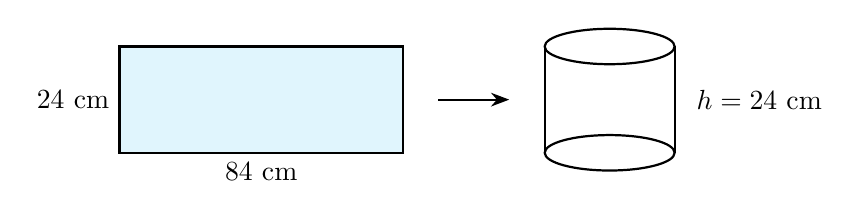
\begin{tikzpicture}[scale=.75]
\draw[fill=lotaCyan!18] (0,0) rectangle (4.8,1.8);
\node[below] at (2.4,0){84 cm};\node[left] at (0,.9){24 cm};
\draw[->,thick] (5.4,.9)--(6.6,.9);
\draw (7.2,0)--(7.2,1.8) (9.4,0)--(9.4,1.8);
\draw (8.3,1.8) ellipse (1.1 and .3);\draw (8.3,0) ellipse (1.1 and .3);
\node[right] at (9.6,.9){$h=24$ cm};
\end{tikzpicture}\par\myndtexti{Skýringarmynd, ekki í kvarða. Plötubreiddin verður ummálið.}
\end{center}
\[U=84\eining{cm},\qquad r=\frac{84}{2\pi}=\frac{42}{\pi}\eining{cm}\approx13{,}37\eining{cm}.\]
Notaðu nákvæma radíusinn í rúmmálsreikningnum:
\[R=\pi\left(\frac{42}{\pi}\right)^2\cdot24=\frac{42336}{\pi}\eining{cm^3}\approx13{,}48\eining{\ell}.\]
Ef plötunni væri rúllað í hina áttina yrði \(h=84\) cm og \(U=24\) cm. Það gæfi annað rúmmál þótt plötuflatarmálið væri óbreytt.
\end{daemi}

\timi{4}{STRÝTUR: PÝRAMÍDAR OG KEILUR}
\markmid{Að reikna rúmmál strýtu, greina hæð frá skáhlið og finna möttul keilu.}
\kafli{Grunnflötur og toppur}
\hugtak{stryta}{Strýta} mjókkar frá grunnfleti að einum toppi. \hugtak{pyramidi}{Pýramídi} hefur marghyrndan grunnflöt og þríhyrnda hliðarfleti. \hugtak{keila}{Keila} hefur hringlaga grunnflöt. Hér er unnið með réttar hringkeilur, þar sem toppurinn er beint yfir miðju hringsins.
\begin{regla}\textbf{FLÝTILEIÐ:} Rúmmál pýramída eða keilu er
\[\tolur{R=\frac{Gh}{3}.}\]
Hæðin \(h\) er alltaf mæld hornrétt á grunnflötinn. Strýta hefur þriðjung af rúmmáli strendings eða sívalnings með sama grunnflöt og sömu hæð.\end{regla}
Grunnflöturinn einn fyllir ekki alla leið upp: þversnið strýtunnar minnka eftir því sem nær dregur toppnum. Stuðullinn \(1/3\) tekur tillit til þessarar mjókkunar.
\begin{center}
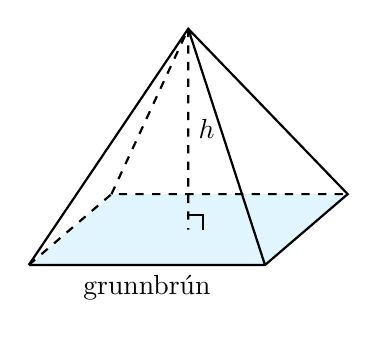
\begin{tikzpicture}[scale=.75]
\coordinate (A) at (0,0);\coordinate (B) at (4,0);\coordinate (C) at (5.4,1.2);\coordinate (D) at (1.4,1.2);\coordinate (T) at (2.7,4);
\fill[lotaCyan!18] (A)--(B)--(C)--(D)--cycle;
\draw (A)--(B)--(C)--(T)--(A) (B)--(T);
\draw[dashed] (A)--(D)--(C) (D)--(T) (T)--node[right]{$h$}(2.7,.6);
\draw (2.7,.85)--(2.95,.85)--(2.95,.6);\node[below] at (2,0){grunnbrún};
\end{tikzpicture}\par\myndtexti{Skýringarmynd í rúmsýn. Strikalínan $h$ er hornrétt hæð pýramídans.}
\end{center}
\begin{daemi}{4.1 · Ferningur eða rétthyrningur í grunni}
Ferningur með hlið \(16\) cm hefur flatarmálið \(256\eining{cm^2}\). Ef pýramídinn er \(21\) cm hár er
\[R=\frac{16^2\cdot21}{3}=1792\eining{cm^3}.\]
Annar pýramídi hefur rétthyrndan grunn \(18\times10\) cm og hæð \(14\) cm. Þá er \(R=(18\cdot10\cdot14)/3=840\eining{cm^3}\).
\end{daemi}
\nyrhluti{Þríhyrndur grunnur og keilur}
\begin{daemi}[lotaCyan]{4.2 · Þríhyrningur í grunni}
Grunnþríhyrningur hefur grunnlínu \(9\) dm og hæð \(4\) dm. Hæð pýramídans er \(15\) dm. Því er
\[G=\frac{9\cdot4}{2}=18\eining{dm^2},\qquad R=\frac{18\cdot15}{3}=90\eining{dm^3}.\]
Deilt er með tveimur vegna þríhyrningsins og með þremur vegna pýramídans.
\end{daemi}

\kafli{Keila: hringflötur í rúmmálsformúlunni}
Fyrir keilu er \(G=\pi r^2\). Setjum það inn í almennu regluna:
\[\tolur{R=\frac{\pi r^2h}{3}.}\]
\begin{center}
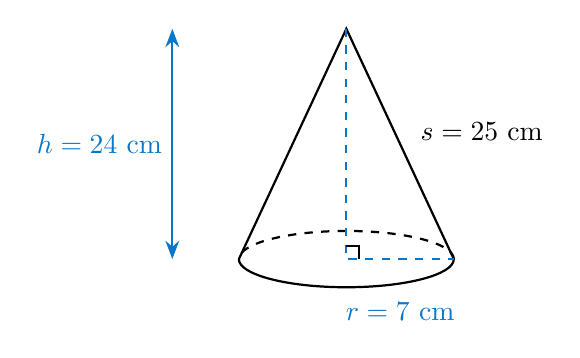
\begin{tikzpicture}[scale=.65]
\coordinate (T) at (0,4.5);\coordinate (O) at (0,0);\coordinate (P) at (2.1,0);
\draw (-2.1,0)--(T)--(P);
\draw (2.1,0) arc[start angle=0,end angle=-180,x radius=2.1,y radius=.55];
\draw[dashed] (2.1,0) arc[start angle=0,end angle=180,x radius=2.1,y radius=.55];
\draw[dashed,lotaBlue] (T)--(O)--node[below=12pt]{$r=7$ cm}(P);
\draw[<->,lotaBlue] (-3.4,0)--node[left]{$h=24$ cm}(-3.4,4.5);
\draw (0,.25)--(.25,.25)--(.25,0);
\node[right] at (1.25,2.5){$s=25$ cm};
\end{tikzpicture}\par\myndtexti{Skýringarmynd, ekki í kvarða. $s$ er skáhlið; hún kemur ekki í stað $h$.}
\end{center}
\begin{daemi}{4.3 · Rúmmál úr radíus og hæð}
Keilan á myndinni hefur rúmmálið
\[R=\frac{\pi\cdot7^2\cdot24}{3}=392\pi\eining{cm^3}\approx1231{,}50\eining{cm^3}.\]
Talan \(25\) á hallandi línunni er ekki hornrétt hæð og á því ekki heima í rúmmálsformúlunni.
\end{daemi}
\begin{daemi}[lotaCyan]{4.4 · Einingar og þvermál}
Keilulaga sandbingur er \(180\) cm hár og \(500\) cm að þvermáli. Í metrum er \(h=1{,}8\) og \(r=2{,}5\).
\[R=\frac{\pi\cdot2{,}5^2\cdot1{,}8}{3}=3{,}75\pi\eining{m^3}\approx11{,}78\eining{m^3}.\]
Lítið keilulaga mæliílát hefur innanþvermálið \(6\) cm og hæðina \(8\) cm. Það rúmar \(24\pi\eining{cm^3}\), eða \(2{,}4\pi\eining{c\ell}\approx7{,}54\eining{c\ell}\). Hvort toppurinn snýr upp eða niður breytir ekki rúmmálinu.
\end{daemi}

\nyrhluti{Skáhlið og möttull keilu}
\hugtak{hallalengd}{Skáhlið} keilu, \(s\), liggur frá toppi eftir möttlinum að jaðri grunnflatar. Í réttum þríhyrningi með hliðar \(r\), \(h\) og \(s\) gildir \(s^2=r^2+h^2\).

Útbreiddur möttull er geiri úr hring með radíus \(s\). Boginn er jafnlangur ummáli grunnhringsins, \(2\pi r\). Möttullinn er því hlutfallið \(r/s\) af hringfleti með flatarmálið \(\pi s^2\): niðurstaðan er \(\pi rs\).
\begin{regla}\textbf{FLÝTILEIÐ:} Möttull keilu: \(M=\pi rs\).\par
Lokuð keila: \(Y=\pi rs+\pi r^2\). \qquad \(s=\sqrt{r^2+h^2}\).\end{regla}
\begin{daemi}[lotaCyan]{4.5 · Opinn keiluhattur}
Keilan í dæmi 4.3 hefur \(s=\sqrt{7^2+24^2}=25\) cm. Í opinn keiluhatt með þessu formi þarf
\[M=\pi\cdot7\cdot25=175\pi\eining{cm^2}\approx549{,}78\eining{cm^2}.\]
Ekki bætist við hringbotn því hatturinn er opinn að neðan.

Í \(80\) smærri skrautkeilur með \(r=3{,}6\) cm og \(s=8{,}5\) cm þarf samtals
\[80\pi\cdot3{,}6\cdot8{,}5=2448\pi\eining{cm^2}\approx0{,}77\eining{m^2},\]
ef skörun og afskurður eru ekki talin með.
\end{daemi}
\kafli{Sama rúmmál í nýju formi}
\begin{daemi}[lotaMagenta]{4.6 · Efni úr pýramída í beinan garðvegg}
Í reiknilíkani er gegnheill pýramídi með ferningsgrunn \(12\times12\) m og hæð \(9\) m tekinn í sundur. Efnið er notað í vegg sem er \(0{,}60\) m breiður og \(1{,}20\) m hár. Gert er ráð fyrir engum holrúmum eða efnistapi.
\[R=\frac{12^2\cdot9}{3}=432\eining{m^3}.\]
Hver metri veggjar notar \(0{,}60\cdot1{,}20=0{,}72\eining{m^3}\), svo
\[L=\frac{432}{0{,}72}=600\eining{m}.\]
\end{daemi}

\nyrhluti{Samsett rúmmál og áætlun um efnisnotkun}
\begin{daemi}{4.7 · Sívalningslaga hylki með keilubotni}
Hylki hefur innanþvermálið \(1{,}2\) m. Sívalningshlutinn er \(1{,}4\) m hár og keilubotninn \(0{,}5\) m hár. Hlutar þess deila grunnhring, en rúmmál þeirra skarast ekki.
\begin{center}
\begin{tikzpicture}[scale=.8]
\draw (-1.5,1.4)--(-1.5,4.2) (1.5,1.4)--(1.5,4.2);
\draw (0,4.2) ellipse(1.5 and .4);
\draw[dashed] (0,1.4) ellipse(1.5 and .4);
\draw (-1.5,1.4)--(0,0)--(1.5,1.4);
\draw[<->] (2,1.4)--node[right]{$1{,}4$ m}(2,4.2);
\draw[<->] (2,0)--node[right]{$0{,}5$ m}(2,1.4);
\draw[<->] (-1.5,4.9)--node[above]{$\text{\th}=1{,}2$ m}(1.5,4.9);
\end{tikzpicture}\par\myndtexti{Skýringarmynd, ekki í kvarða.}
\end{center}
\[\begin{aligned}
R&=\pi\cdot0{,}6^2\cdot1{,}4+\frac{\pi\cdot0{,}6^2\cdot0{,}5}{3}\\
&=0{,}504\pi+0{,}060\pi=0{,}564\pi\eining{m^3}\approx1771{,}86\eining{\ell}.
\end{aligned}\]
\end{daemi}
\begin{daemi}[lotaMagenta]{4.8 · Hve margar keilur má áætla úr efni?}
Skrautkeila án botns er \(8\) cm að þvermáli og \(15\) cm há. Fyrst finnum við skáhliðina:
\[s=\sqrt{4^2+15^2}=\sqrt{241}\eining{cm},\qquad M=4\pi\sqrt{241}\eining{cm^2}.\]
Efnisbútur er \(50\times90\) cm, alls \(4500\eining{cm^2}\). Hlutfallið er
\[\frac{4500}{4\pi\sqrt{241}}\approx23{,}07.\]
Flatarmálið nægir í \textbf{að hámarki 23 heilar keilur}. Það er efri mörk út frá flatarmáli; raunverulegur fjöldi getur verið minni vegna lögunar sniðanna, samskeyta og afskurðar.
\end{daemi}

\timi{5}{KÚLUR}
\markmid{Að reikna rúmmál og yfirborð kúlu og hálfkúlu, bera saman massa og finna fjölda við endurmótun.}
\kafli{Radíusinn ræður stærð kúlunnar}
Allir punktar á yfirborði \hugtak{kula}{kúlu} eru jafnlangt frá miðju hennar. Sú fjarlægð er radíus \(r\). Þvermálið er \(2r\), eins og í hring.
\begin{center}
\begin{tikzpicture}[scale=.85]
\draw[fill=lotaCyan!10] (0,0) circle(1.65);
\draw (1.65,0) arc[start angle=0,end angle=-180,x radius=1.65,y radius=.43];
\draw[dashed] (1.65,0) arc[start angle=0,end angle=180,x radius=1.65,y radius=.43];
\fill (0,0) circle(1.5pt);\draw[lotaBlue,thick] (0,0)--node[above]{$r$}(1.65,0);
\node[right,align=left] at (2.6,.3){Rúmmál: $\displaystyle R=\frac43\pi r^3$\\[12pt]Yfirborð: $Y=4\pi r^2$};
\end{tikzpicture}\par\myndtexti{Skýringarmynd af kúlu. Strikalínan sýnir falinn hluta miðbaugs.}
\end{center}
\begin{regla}\textbf{FLÝTILEIÐ:} Kúla: \(R=\frac43\pi r^3\).\par
\hugtak{halfkula}{Hálfkúla}: \(R=\frac12\cdot\frac43\pi r^3=\frac23\pi r^3\).\end{regla}
Rúmmál kúlu er tveir þriðju af rúmmáli sívalnings með sama radíus og hæð \(2r\). Þetta hjálpar að tengja regluna við \(\pi r^2\cdot2r\), en yfirborðsformúlan er önnur regla.
\begin{daemi}{5.1 · Radíus gefinn}
Gegnheil kúla hefur radíus \(4\) cm.
\[R=\frac43\pi\cdot4^3=\frac{256\pi}{3}\eining{cm^3}\approx268{,}08\eining{cm^3}.\]
Reiknaðu \(4^3=64\) áður en margfaldað er með \(4\pi/3\).
\end{daemi}
\begin{daemi}[lotaCyan]{5.2 · Þvermál gefið og svar í lítrum}
Kúlulaga sýningarbelgur er \(0{,}90\) m að innanþvermáli, svo \(r=0{,}45\) m.
\[R=\frac43\pi\cdot0{,}45^3=0{,}1215\pi\eining{m^3}=121{,}5\pi\eining{\ell}\approx381{,}70\eining{\ell}.\]
\end{daemi}
\nyrhluti{Hálfkúlur og yfirborðsflatarmál}
\begin{daemi}[lotaMagenta]{5.3 · Rými í hálfkúlu}
Hálfkúlulaga tjald hefur innanþvermálið \(3{,}6\) m.
\[R=\frac23\pi\cdot1{,}8^3=3{,}888\pi\eining{m^3}\approx12{,}21\eining{m^3}.\]
Hér er aðeins reiknað rýmið inni í tjaldinu, ekki efni í dúkinn.
\end{daemi}

\kafli{Yfirborð kúlu og hálfkúlu}
Yfirborðsflatarmál kúlu er fjórfalt flatarmál hrings með sama radíus. Bogið yfirborð hálfkúlu er helmingur þess. Ef hálfkúlan hefur líka flatan botn þarf að bæta einum hringfleti við.
\begin{regla}\textbf{FLÝTILEIÐ:}\par
Kúla: \(Y=4\pi r^2\).\par
Bogið yfirborð hálfkúlu: \(Y_{\text{bogið}}=2\pi r^2\).\par
Hálfkúla með flötum botni: \(Y_{\text{allt}}=3\pi r^2\).\end{regla}
\begin{daemi}{5.4 · Efni utan um kúlu}
Kúlulaga lampaskermur hefur radíus \(22\) cm, eða \(0{,}22\) m. Ef reiknað er með heilli kúlu þarf
\[Y=4\pi\cdot0{,}22^2=0{,}1936\pi\eining{m^2}\approx0{,}61\eining{m^2}.\]
Formúlan er sú sama fyrir stórar kúlur: í líkani er ímyndað tungl \(2600\) km að þvermáli, svo yfirborðið er
\[Y=4\pi\cdot1300^2=6760000\pi\eining{km^2}\approx21237166\eining{km^2}.\]
\end{daemi}
\begin{daemi}[lotaMagenta]{5.5 · Hálfkúlulaga þak með viðbót}
Hálfkúlulaga þak er \(7{,}6\) m að þvermáli. Þekja á bogna flötinn og bæta \(12\%\) við vegna samskeyta og afskurðar.
\skref{1} Radíusinn er \(3{,}8\) m. Bogna yfirborðið er
\[Y_{\text{bogið}}=2\pi\cdot3{,}8^2=28{,}88\pi\eining{m^2}.\]
\skref{2} Viðbótin gefur margföldunarstuðulinn \(1{,}12\):
\[F_{\text{efni}}=1{,}12\cdot28{,}88\pi=32{,}3456\pi\eining{m^2}\approx101{,}62\eining{m^2}.\]
Flati grunnhringurinn er ekki hluti þaksins sem á að þekja.
\end{daemi}

\nyrhluti{Endurmótun og samanburður á massa}
\begin{daemi}{5.6 · Ein kúla verður að mörgum smærri}
Vaxkúla er \(6\) cm að þvermáli. Hún er brædd og mótuð í litlar kúlur, \(3\) mm að þvermáli. Gerum ráð fyrir engu tapi og óbreyttum eðlismassa.
\skref{1} Samræmdu einingar: \(6\eining{cm}=60\eining{mm}\). Hlutfall þvermálanna er \(60/3=20\), og radíusarnir hafa sama hlutfall.
\skref{2} Rúmmálshlutfallið er teningur lengdarhlutfallsins:
\[N=\frac{R_{\text{stór}}}{R_{\text{lítil}}}=\frac{\frac43\pi r_{\text{stór}}^3}{\frac43\pi r_{\text{lítil}}^3}=20^3=8000.\]
Úr stóru kúlunni fást \(8000\) litlar kúlur við þessar forsendur.
\end{daemi}
\begin{mundu}\textbf{MUNDU:} Ekki deila þvermálunum og kalla það fjölda kúlna. Rúmmál breytist með þriðja veldi lengdar, ekki fyrsta veldi.\end{mundu}
\begin{daemi}[lotaMagenta]{5.7 · Stærri kúla úr léttara efni}
Í reiknilíkani eru tvö efni, A og B. Hver cm\(^3\) af A vegur \(7{,}5\) g en hver cm\(^3\) af B vegur \(2{,}4\) g. Kúla A er \(1{,}6\) cm að þvermáli og kúla B \(2{,}4\) cm.
\[\begin{aligned}
m_A&=7{,}5\cdot\frac43\pi\cdot0{,}8^3=5{,}12\pi\eining{g}\approx16{,}08\eining{g},\\
m_B&=2{,}4\cdot\frac43\pi\cdot1{,}2^3=5{,}5296\pi\eining{g}\approx17{,}37\eining{g}.
\end{aligned}\]
Kúla B er þyngri þótt efnið í henni hafi minni eðlismassa.

Önnur leið er að bera massana saman með hlutfalli:
\[\frac{m_B}{m_A}=\frac{2{,}4}{7{,}5}\left(\frac{1{,}2}{0{,}8}\right)^3=1{,}08.\]
Kúla B hefur \(8\%\) meiri massa. Stærð og eðlismassi skipta bæði máli.
\end{daemi}
\kafli{Veldu spurninguna áður en þú velur formúluna}
\begin{itemize}
\item Rými eða magn efnis inni í kúlu: \(R=\frac43\pi r^3\).
\item Dúkur, plast eða málning á yfirborði: \(Y=4\pi r^2\).
\item Massi: reiknaðu rúmmál og margfaldaðu með eðlismassa.
\item Fjöldi við endurmótun: deildu heildarrúmmáli með rúmmáli eins hlutar.
\end{itemize}

\timi{6}{HAGNÝT DÆMI I}
\markmid{Að velja formúlu út frá lögun, reikna samsett form, finna óþekkta hæð og tengja stærðarhlutföll við prósentur.}
\kafli{Lesa myndina áður en reiknað er}
Byrjaðu á að nefna formið, merkja grunnflötinn og finna hornrétta hæð. Spurðu síðan hvort leitað sé að rúmmáli eða flatarmáli. Ef hringur kemur við sögu þarf að vita hvort gefna lengdin er radíus eða þvermál.
\begin{daemi}{6.1 · Sex form, sex uppsetningar}
Hér eru nýjar stærðir fyrir form sem þú þekkir. Allar hæðir í töflunni eru hornréttar hæðir.
\renewcommand{\arraystretch}{1.4}
\begin{tabularx}{\linewidth}{@{}>{\raggedright\arraybackslash}p{.27\linewidth} >{\raggedright\arraybackslash}X@{}}
\toprule\textbf{Form og mál}&\textbf{Uppsetning og rúmmál}\\\midrule
Ferstrendingur: \(240\times90\times65\) mm&\(R=240\cdot90\cdot65=1404000\eining{mm^3}\), eða \(1404\eining{cm^3}\).\\
Pýramídi: ferningshlið \(14\) dm, \(h=18\) dm&\(R=14^2\cdot18/3=1176\eining{dm^3}\).\\
Þrístrendingur: skammhliðar \(5\) og \(12\) cm, lengd \(8\) cm&\(G=5\cdot12/2=30\eining{cm^2}\), svo \(R=30\cdot8=240\eining{cm^3}\).\\
Keila: \(\text{\th}=14\) m, \(h=9\) m&\(r=7\) m, svo \(R=\pi\cdot7^2\cdot9/3=147\pi\eining{m^3}\).\\
Sívalningur: \(r=0{,}7\) m, \(h=1{,}6\) m&\(R=\pi\cdot0{,}7^2\cdot1{,}6=0{,}784\pi\eining{m^3}\).\\
Kúla: \(r=9\) cm&\(R=\frac43\pi\cdot9^3=972\pi\eining{cm^3}\).\\\bottomrule
\end{tabularx}
\end{daemi}
\begin{daemi}[lotaCyan]{6.2 · Flatarmál er önnur spurning}
Teningur með brún \(3{,}2\) cm hefur yfirborðið
\[Y=6\cdot3{,}2^2=61{,}44\eining{cm^2}.\]
Sívalningur með \(\text{\th}=18\) cm og \(h=7\) cm hefur möttulinn
\[M=\pi\text{\th}h=\pi\cdot18\cdot7=126\pi\eining{cm^2}.\]
Hvorugt þessara svara er rúmmál. Í seinna svarinu eru hringlaga endafletirnir ekki taldir með.
\end{daemi}

\nyrhluti{Skiptu samsettum hlut í þekkt form}
\begin{daemi}[lotaCyan]{6.3 · Hálfur sívalningur sem skýli}
Skýli er hálfur liggjandi sívalningur, \(12\) m langt og \(5\) m breitt við jörð. Báðir hálfhringlaga endar eru lokaðir með dúk. Enginn dúkur fer í gólf og op fyrir dyr eru ekki dregin frá.
\begin{center}
\begin{tikzpicture}[scale=.65]
\draw[fill=lotaCyan!15] (-2.5,0) arc[start angle=180,end angle=0,radius=2.5]--cycle;
\draw (1.5,1.6) arc[start angle=180,end angle=0,radius=2.5];
\draw (-2.5,0)--(1.5,1.6) (2.5,0)--(6.5,1.6) (0,2.5)--(4,4.1);
\draw[dashed] (1.5,1.6)--(6.5,1.6);
\node[below] at (0,0){$\text{\th}=5$ m};\node[below right] at (4.5,.8){$L=12$ m};
\end{tikzpicture}\par\myndtexti{Skýringarmynd í rúmsýn, ekki í kvarða.}
\end{center}
\skref{1} Radíusinn er \(2{,}5\) m. Rúmmálið er hálft sívalningsrúmmál:
\[R=\frac12\pi\cdot2{,}5^2\cdot12=37{,}5\pi\eining{m^3}\approx117{,}81\eining{m^3}.\]
\skref{2} Bogni dúkurinn er hálfur möttull. Tveir hálfhringir mynda einn hring:
\[F_{\text{dúkur}}=\pi\cdot2{,}5\cdot12+\pi\cdot2{,}5^2
=36{,}25\pi\eining{m^2}\approx113{,}88\eining{m^2}.\]
\end{daemi}
\begin{daemi}[lotaMagenta]{6.4 · Sívalningur með hálfkúlu ofan á}
Líkan af turni hefur radíus \(3\) cm. Sívalningshlutinn er \(7\) cm hár og ofan á honum er hálfkúla með sama radíus.
\[R=\pi\cdot3^2\cdot7+\frac23\pi\cdot3^3=63\pi+18\pi=81\pi\eining{cm^3}.\]
Rúmmálið er um \(254{,}47\eining{cm^3}\). Heildarhæð líkansins er \(7+3=10\) cm, en hæð sívalningsins í formúlunni er aðeins \(7\) cm.
\end{daemi}
\begin{mundu}\textbf{MUNDU:} Rúmmál samsetts hlutar fæst með samlagningu þegar hlutarnir skarast ekki. Við yfirborðsreikning þarf sérstaklega að finna hvaða fletir eru faldir inni í hlutnum.\end{mundu}

\nyrhluti{Rúmmál þekkt, hæð óþekkt}
Til að einangra óþekkta stærð gerum við sömu aðgerð báðum megin jafnaðarmerkis. Þegar \(G>0\) fæst úr \(R=Gh\):
\[\frac{R}{G}=h.\]
Fyrir strýtu þarf fyrst að margfalda með þremur: \(3R=Gh\), svo \(h=3R/G\).
\begin{regla}\textbf{FLÝTILEIÐ:}\par
Strendingur eða sívalningur: \(h=R/G\).\par
Pýramídi eða keila: \(h=3R/G\). Hér er \(G>0\).\end{regla}
\begin{daemi}{6.5 · Hækkun vatnsborðs}
Sívalningslaga ílát hefur innanþvermálið \(1{,}6\) m. Í það er bætt \(2{,}4\eining{m^3}\) af vatni. Hækkunin er hæð viðbótarvatnsins, að því gefnu að vatn leki ekki út eða flæði yfir.
\[G=\pi\cdot0{,}8^2=0{,}64\pi\eining{m^2},\qquad
\Delta h=\frac{2{,}4}{0{,}64\pi}=\frac{3{,}75}{\pi}\eining{m}\approx1{,}19\eining{m}.\]
Prófun: \(0{,}64\pi\cdot(3{,}75/\pi)=2{,}4\eining{m^3}\).
\end{daemi}
\begin{daemi}[lotaCyan]{6.6 · Hæð íláts úr rúmmáli}
Sívalningslaga ílát er \(7\) cm að innanþvermáli og rúmar \(42\) c\(\ell\). Fyrst er \(42\eining{c\ell}=420\eining{cm^3}\).
\[h=\frac{420}{\pi\cdot3{,}5^2}\eining{cm}\approx10{,}91\eining{cm}.\]
Sé rúmmálið \(70\) c\(\ell\) við sama þvermál fæst í staðinn
\[h=\frac{700}{\pi\cdot3{,}5^2}\eining{cm}\approx18{,}19\eining{cm}.\]
Við fastan grunnflöt breytist hæð í sama hlutfalli og rúmmál.
\end{daemi}
\begin{daemi}[lotaMagenta]{6.7 · Hæð pýramída}
Pýramídi hefur ferningsgrunn með hlið \(9\) cm og rúmmálið \(405\eining{cm^3}\).
\[h=\frac{3R}{G}=\frac{3\cdot405}{9^2}=15\eining{cm}.\]
Prófun: \(9^2\cdot15/3=405\eining{cm^3}\).
\end{daemi}

\nyrhluti{Frá ummáli að rúmmáli}
\begin{daemi}{6.8 · Ummál grunnhringsins er gefið}
Sívalningur er \(7\) cm hár og ummál grunnflatar er \(31{,}4\) cm.
\skref{1} Einangraðu radíusinn:
\[r=\frac{U}{2\pi}=\frac{31{,}4}{2\pi}\eining{cm}.\]
\skref{2} Settu nákvæmu stæðuna inn í rúmmálsformúluna:
\[R=\pi\left(\frac{31{,}4}{2\pi}\right)^2\cdot7
=\frac{7\cdot31{,}4^2}{4\pi}\eining{cm^3}\approx549{,}22\eining{cm^3}.\]
Ekki nota ummálið sem radíus eða þvermál. Báðar þær lengdir eru minni en ummálið.
\end{daemi}
\kafli{Prósentubreyting á lengd, flatarmáli og rúmmáli}
\begin{daemi}[lotaMagenta]{6.9 · Allar brúnir lengjast um 15\%}
Allar brúnir tenings eru lengdar um \(15\%\), svo \(k=1{,}15\).
\[\frac{Y_{\text{nýtt}}}{Y_{\text{gamalt}}}=k^2=1{,}3225.\]
Nýja yfirborðið er \(132{,}25\%\) af því gamla og \textbf{aukningin} er því \(32{,}25\%\).
\[\frac{R_{\text{nýtt}}}{R_{\text{gamalt}}}=k^3=1{,}520875.\]
Nýja rúmmálið er \(152{,}0875\%\) af því gamla og aukningin er \(52{,}0875\%\), eða um \(52{,}09\%\).
\end{daemi}
\begin{regla}\textbf{FLÝTILEIÐ:} Ef allar lengdir breytast með stuðlinum \(k>0\):
\[\text{breyting á flatarmáli}=(k^2-1)\cdot100\%,\]
\[\text{breyting á rúmmáli}=(k^3-1)\cdot100\%.\]
Neikvæð niðurstaða merkir minnkun.\end{regla}
\begin{mundu}\textbf{ATH.:} Þessar reglur gilda þegar \emph{allar} lengdir breytast í sama hlutfalli. Ef aðeins hæð sívalnings tvöfaldast, tvöfaldast rúmmálið. Ef bæði radíus og hæð tvöfaldast, áttfaldast það.\end{mundu}

\timi{7}{HAGNÝT DÆMI II}
\markmid{Að finna hlutföll og óþekktar lengdir, nota Pýþagóras í rúmmyndum og reikna yfirborð samsettra hluta.}
\kafli{Hlutföll: hvað breytist og hvað helst?}
\begin{daemi}{7.1 · Rúmmálshlutfall tveggja teninga}
Teningar hafa brúnir \(9\) cm og \(6\) cm. Lengdarhlutfallið, stærri á móti minni, er \(9:6=3:2\). Rúmmálshlutfallið er
\[\frac{R_{\text{stærri}}}{R_{\text{minni}}}=\left(\frac{3}{2}\right)^3=\frac{27}{8}.\]
Það má skrifa \(27:8\). Stærri teningurinn hefur \(3{,}375\) sinnum rúmmál þess minni.
\end{daemi}
\begin{daemi}[lotaCyan]{7.2 · Mismunandi radíus og hæð}
Sívalningur A hefur \(r=3\) cm og \(h=20\) cm. Sívalningur B hefur \(r=5\) cm og \(h=12\) cm.
\[R_A=180\pi\eining{cm^3},\qquad R_B=300\pi\eining{cm^3}.\]
Sívalningur B hefur meira rúmmál þótt hann sé lægri. Hlutfallið er
\[\frac{R_B}{R_A}=\frac{300\pi}{180\pi}=\frac53,\quad\text{þ.e.}\quad5:3.\]
Sívalningarnir eru ekki einslaga; berðu saman \(r^2h\) fyrir hvorn þeirra.
\end{daemi}
\kafli{Óþekktur radíus}
\begin{daemi}[lotaMagenta]{7.3 · Rúmmál og hæð gefin}
Sívalningslaga ílát er \(16\) cm hátt og rúmar \(0{,}75\) lítra, eða \(750\eining{cm^3}\).
\[750=\pi r^2\cdot16\quad\Longrightarrow\quad r^2=\frac{750}{16\pi}.\]
Tökum jákvæða ferningsrót vegna þess að radíus er lengd:
\[\tolur{r=\sqrt{\frac{750}{16\pi}}\eining{cm}\approx3{,}86\eining{cm}.}\]
Þvermálið væri um \(7{,}73\) cm. Spurt var um radíus, svo það er fyrra svarið sem við skilum.

\textbf{Mundu:} Úr \(r^2=A\) fæst \(r=\sqrt A\) fyrir jákvæða lengd, ekki \(r=A/2\).
\end{daemi}

\nyrhluti{Pýþagóras áður en rúmmál er reiknað}
Finndu rétthyrndan þríhyrning í myndinni. Langhliðin liggur á móti rétta horninu og uppfyllir \(c^2=a^2+b^2\). Þegar skammhlið vantar drögum við hinn ferninginn frá.
\begin{daemi}{7.4 · Radíus keilu úr hæð og skáhlið}
Rétt keila hefur hæð \(40\) cm og skáhlið \(41\) cm. Þríhyrningurinn frá toppi að miðju og jaðri grunnflatar gefur:
\begin{center}
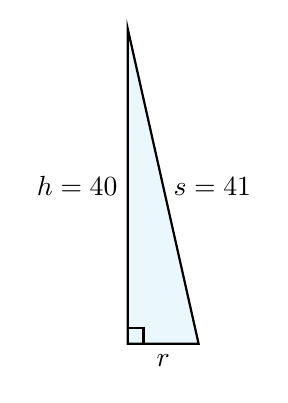
\begin{tikzpicture}[x=.10cm,y=.10cm]
\draw[fill=lotaCyan!12] (0,0)--(9,0)--(0,40)--cycle;
\draw (0,2)--(2,2)--(2,0);
\node[left] at (0,20){$h=40$};\node[below] at (4.5,0){$r$};\node[right] at (4.5,20){$s=41$};
\end{tikzpicture}\par\myndtexti{Þríhyrningur innan keilunnar. Allar lengdir eru í cm.}
\end{center}
\[r^2=41^2-40^2=81,\qquad r=9\eining{cm}.\]
Nú fæst rúmmálið:
\[R=\frac{\pi\cdot9^2\cdot40}{3}=1080\pi\eining{cm^3}.\]
\end{daemi}
\begin{daemi}[lotaCyan]{7.5 · Hornalína í þversniði sívalnings}
Lóðrétt snið gegnum miðju sívalnings er rétthyrningur. Hæð þess er \(24\) cm og hornalína \(25\) cm. Breidd sniðsins er \textbf{þvermál}, ekki radíus.
\begin{center}
\begin{tikzpicture}[x=.15cm,y=.15cm]
\draw[fill=lotaCyan!12] (0,0) rectangle (7,24);
\draw[lotaBlue,thick] (0,24)--(7,0);
\node[right,lotaBlue] at (10,12){$25$};\draw[->,lotaBlue] (10,12)--(3.5,12);
\node[left] at (0,12){$24$};\node[below] at (3.5,0){$\text{\th}$};
\draw (0,1.5)--(1.5,1.5)--(1.5,0);
\end{tikzpicture}
\end{center}
\[\text{\th}=\sqrt{25^2-24^2}=7\eining{cm},\qquad r=3{,}5\eining{cm}.\]
\[R=\pi\cdot3{,}5^2\cdot24=294\pi\eining{cm^3}.\]
\end{daemi}

\nyrhluti{Hæð hliðarflatar og óþekktar grunnbrúnir}
\begin{daemi}[lotaMagenta]{7.6 · Yfirborð reglulegs ferningspýramída}
Grunnbrún pýramída er \(20\) cm og hver hliðarbrún frá toppi að grunnhorni er \(26\) cm. Toppurinn er beint yfir miðju ferningsins. Fjórir hliðarfletir eru því eins jafnarma þríhyrningar.
\begin{center}
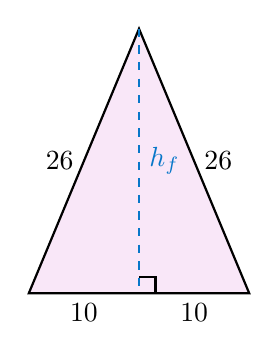
\begin{tikzpicture}[x=.14cm,y=.14cm]
\draw[fill=lotaMagenta!15] (-10,0)--(10,0)--(0,24)--cycle;
\draw[dashed,lotaBlue] (0,24)--node[right]{$h_f$}(0,0);
\draw (0,1.5)--(1.5,1.5)--(1.5,0);
\node[below] at (-5,0){10};\node[below] at (5,0){10};
\node[right] at (5,12){26};\node[left] at (-5,12){26};
\end{tikzpicture}\par\myndtexti{Einn hliðarflötur. Allar lengdir eru í cm.}
\end{center}
Hæð \emph{hliðarflatarins} er \(h_f=\sqrt{26^2-10^2}=24\) cm. Hún er ekki lóðrétt hæð pýramídans.
\[Y=20^2+4\left(\frac{20\cdot24}{2}\right)=400+960=1360\eining{cm^2}.\]
\end{daemi}
\begin{daemi}{7.7 · Jafna fyrir grunnbrúnir kassa}
Grunnbrúnir kassa eru \(x\) cm og \(3x\) cm. Hæðin er \(10\) cm og rúmmálið \(1470\eining{cm^3}\).
\[x\cdot3x\cdot10=1470\quad\Longrightarrow\quad30x^2=1470\quad\Longrightarrow\quad x^2=49.\]
Þar sem \(x>0\) er \(x=7\). Grunnbrúnirnar eru því \(7\) cm og \(21\) cm. Prófun: \(7\cdot21\cdot10=1470\).
\end{daemi}
\begin{daemi}[lotaCyan]{7.8 · Rúmmál tenings úr flatarmáli}
Ef grunnflatarmál tenings er \(81\eining{cm^2}\), er \(s=\sqrt{81}=9\) cm og \(R=9^3=729\eining{cm^3}\).

Ef \emph{heildaryfirborðið} er \(864\eining{cm^2}\), deilum við fyrst með sex:
\[s^2=864/6=144,\qquad s=12\eining{cm},\qquad R=1728\eining{cm^3}.\]
\end{daemi}

\nyrhluti{Hornalína gegnum kassa}
Hornalína í kassa tengir tvö gagnstæð horn í ferstrendingi og liggur í gegnum hann. Við finnum hana með því að nota Pýþagóras tvisvar.
\begin{daemi}{7.9 · Lengsta beina stöngin í kassanum}
Kassi hefur innanmálin \(12\times9\times20\) cm. Punktarnir \(A\) og \(C\) eru gagnstæð horn botnsins. \(D\) er beint yfir \(C\).
\begin{center}
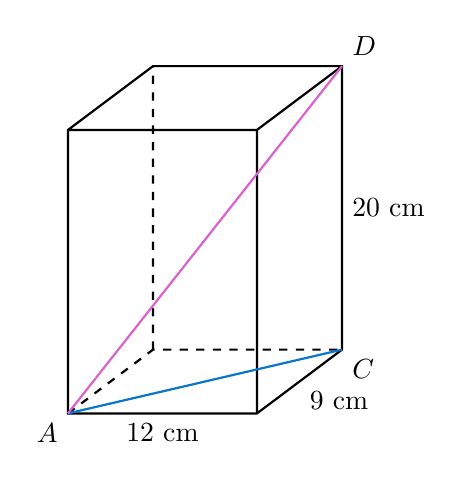
\begin{tikzpicture}[scale=.6]
\coordinate(A)at(0,0);\coordinate(B)at(4,0);\coordinate(C)at(5.8,1.35);\coordinate(E)at(1.8,1.35);
\coordinate(F)at(0,6);\coordinate(G)at(4,6);\coordinate(D)at(5.8,7.35);\coordinate(H)at(1.8,7.35);
\draw(A)--(B)--(C)--(D)--(H)--(F)--cycle (F)--(G)--(D) (B)--(G);
\draw[dashed](A)--(E)--(C) (E)--(H);
\draw[lotaBlue,thick](A)--(C);\draw[lotaMagenta,thick](A)--(D);
\node[below left]at(A){$A$};\node[below right]at(C){$C$};\node[above right]at(D){$D$};
\node[below]at(2,0){12 cm};\node[below right]at(4.9,.675){9 cm};\node[right]at(5.8,4.35){20 cm};
\end{tikzpicture}\par\myndtexti{Skýringarmynd í rúmsýn. Blá lína er hornalína botns; fjólublá lína er hornalína í kassa.}
\end{center}
\[AC=\sqrt{12^2+9^2}=15\eining{cm},\qquad AD=\sqrt{15^2+20^2}=25\eining{cm}.\]
Því kemst \(25\) cm löng stöng í kassann ef hún er hugsuð án þykktar. Almennt er \(d=\sqrt{a^2+b^2+h^2}\).
\end{daemi}
\begin{mundu}\textbf{MUNDU:} Hornalína eins flatar og hornalína í kassa eru ekki sama lengdin. Mesta fjarlægð milli punkta í rétthyrndum kassa liggur milli gagnstæðra horna.\end{mundu}

\nyrhluti{Ytra yfirborð: sameiginlegur flötur telst ekki með}
Þegar tveir hlutir eru festir saman hverfur snertiflöturinn inn í heildina. Teldu þá aðeins þá fleti sem sjást utan á hlutnum. Sameiginlegur hringflötur bætist ekki við ytra yfirborðið.
\begin{daemi}[lotaMagenta]{7.10 · Keila fest á hálfkúlu}
Keila og hálfkúla deila sama grunnhring. Keilan er \(12\) cm há og skáhliðin er \(13\) cm. Finna á yfirborðsflatarmál alls hlutarins.
\begin{center}
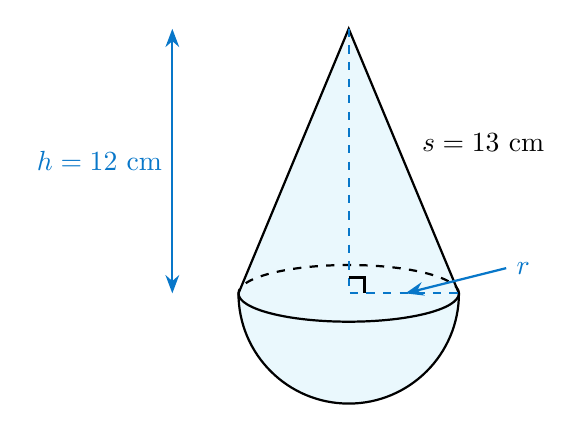
\begin{tikzpicture}[scale=.8]
\draw[fill=lotaCyan!12] (-1.75,0)--(0,4.2)--(1.75,0) arc[start angle=0,end angle=-180,radius=1.75]--cycle;
\draw (1.75,0) arc[start angle=0,end angle=-180,x radius=1.75,y radius=.45];
\draw[dashed] (1.75,0) arc[start angle=0,end angle=180,x radius=1.75,y radius=.45];
\draw[dashed,lotaBlue] (0,4.2)--(0,0)--(1.75,0);
\draw[<->,lotaBlue] (-2.8,0)--node[left]{$h=12$ cm}(-2.8,4.2);
\node[right,lotaBlue] at (2.5,.4){$r$};\draw[->,lotaBlue] (2.5,.4)--(.9,0);
\draw (0,.25)--(.25,.25)--(.25,0);\node[right] at (1,2.4){$s=13$ cm};
\end{tikzpicture}\par\myndtexti{Skýringarmynd í rúmsýn. Hringflöturinn á samskeytunum er inni í hlutnum.}
\end{center}
\skref{1} Finndu sameiginlega radíusinn:
\[r=\sqrt{13^2-12^2}=5\eining{cm}.\]
\skref{2} Leggðu saman möttul keilu og bogið yfirborð hálfkúlu:
\[Y=\pi rs+2\pi r^2=\pi\cdot5\cdot13+2\pi\cdot5^2
=115\pi\eining{cm^2}\approx361{,}28\eining{cm^2}.\]
\skref{3} Athugaðu flatalistann: einn keilumöttull og einn boginn hálfkúluflötur. Enginn flatur hringbotn er að utan.
\end{daemi}
\begin{regla}\textbf{FLÝTILEIÐ:} Skrifaðu lista yfir ytri fleti áður en þú setur saman yfirborðsformúlu. Við samsetningu tveggja lokaðra hluta má einnig leggja saman yfirborðin og draga snertiflötinn frá \emph{tvisvar}, því hann var talinn með í báðum hlutum.\end{regla}

\clearpage\phantomsection\label{gatlisti}
\begin{center}{\fontsize{20}{24}\selectfont\bfseries GÁTLISTI LOTU 29}\end{center}
Merktu við þegar þú getur útskýrt aðferðina og notað hana sjálfstætt. Ef eitthvað er óljóst geturðu smellt á tímanúmerið og rifjað upp.
\kafli{\hyperref[timi:lota29-01]{1. tími · Ferstrendingar}}
\gat{Ég get reiknað rúmmál ferstrendings og breytt svarinu í lítra.}
\gat{Ég get fundið yfirborðsflatarmál lokaðs kassa og greint það frá rúmmáli.}
\gat{Ég get lesið brúnarlengd úr sniði tenings og fundið rúmmál og yfirborð.}
\gat{Ég get notað rúmmál til að reikna massa eða hlutfallslegt magn.}
\gat{Ég get borið saman rúmmál, umbúðaefni og kostnað einslaga kassa.}
\kafli{\hyperref[timi:lota29-02]{2. tími · Strendingar}}
\gat{Ég get greint grunnflöt og hornrétta hæð strendings á mynd.}
\gat{Ég get reiknað rúmmál þrístrendings, möttul hans og heildaryfirborð.}
\gat{Ég get skipt þversniði tröppu, rásar eða húss í einfaldari fleti.}
\gat{Ég get fundið rúmmál laugar með hallandi botni.}
\gat{Ég get reiknað botn og veggi sitt í hvoru lagi og greint lengd eftir halla frá láréttri lengd.}
\kafli{\hyperref[timi:lota29-03]{3. tími · Sívalningar}}
\gat{Ég get notað radíus eða þvermál til að finna rúmmál sívalnings.}
\gat{Ég get útskýrt hvers vegna möttull sívalnings hefur flatarmálið \(2\pi rh\).}
\gat{Ég get reiknað heildarefni, málningarmagn og kostnað í heilum dósum.}
\gat{Ég get samræmt einingar í dæmi um þunnt lag.}
\gat{Ég get fundið radíus og rúmmál þegar plata verður að sívalningsmöttli.}
\kafli{\hyperref[timi:lota29-04]{4. tími · Strýtur}}
\gat{Ég get reiknað rúmmál pýramída með ferhyrndum eða þríhyrndum grunni.}
\gat{Ég get reiknað rúmmál keilu og breytt á milli rúmeininga og lítra eða sentilítra.}
\gat{Ég get greint hornrétta hæð frá skáhlið og reiknað möttul keilu.}
\gat{Ég get lagt saman rúmmál sívalnings og keilu og notað rúmmál við endurmótun.}
\gat{Ég get útskýrt hvers vegna flatarmál eitt tryggir ekki nákvæman fjölda útklipptra hluta.}

\newpage
\kafli{\hyperref[timi:lota29-05]{5. tími · Kúlur}}
\gat{Ég get reiknað rúmmál kúlu og hálfkúlu úr radíus eða þvermáli.}
\gat{Ég get greint milli yfirborðs kúlu, bogins hálfkúluflatar og hálfkúlu með botni.}
\gat{Ég get bætt prósentuviðbót við reiknað efnismagn.}
\gat{Ég get fundið fjölda lítilla kúlna sem fást við endurmótun stærri kúlu.}
\gat{Ég get borið saman massa kúlna með ólíka stærð og eðlismassa.}
\kafli{\hyperref[timi:lota29-06]{6. tími · Hagnýt dæmi I}}
\gat{Ég get valið rúmmálsformúlu út frá lögun og merkingum á mynd.}
\gat{Ég get reiknað rúmmál og dúk í hálfsívalningslaga skýli með skýrum forsendum.}
\gat{Ég get reiknað rúmmál sívalnings með hálfkúlu ofan á.}
\gat{Ég get einangrað hæð í rúmmálsformúlu og prófað með innsetningu.}
\gat{Ég get farið frá ummáli að radíus og áfram að rúmmáli sívalnings.}
\gat{Ég get fundið prósentubreytingu flatarmáls og rúmmáls þegar allar lengdir breytast.}
\kafli{\hyperref[timi:lota29-07]{7. tími · Hagnýt dæmi II}}
\gat{Ég get borið saman rúmmál teninga og sívalninga og stytt hlutföll.}
\gat{Ég get fundið radíus sívalnings úr rúmmáli og hæð.}
\gat{Ég get notað Pýþagóras til að finna óþekktan radíus, þvermál eða hæð hliðarflatar.}
\gat{Ég get reiknað yfirborð reglulegs ferningspýramída úr grunnbrún og hliðarbrún.}
\gat{Ég get sett upp jöfnu fyrir óþekktar grunnbrúnir og valið jákvæða lengd.}
\gat{Ég get fundið rúmmál tenings út frá grunnflatarmáli eða heildaryfirborði.}
\gat{Ég get reiknað hornalínu botns og hornalínu í kassa.}
\gat{Ég get reiknað ytra yfirborð samsetts hlutar án þess að telja innri snertiflöt með.}
\bigskip
\kafli{Um efnið}
Efnisval og tímaskipting byggjast á verkefnablöðum kennara, \emph{29.1 dæmi.pdf} til \emph{29.7 dæmi.pdf}, fyrir 10. bekk. Sýnidæmin í þessu hefti eru samin sérstaklega með nýjum tölum og aðstæðum. Þau eru ekki lausnir verkefnablaðanna.

\clearpage\phantomsection\label{hugtok}
\begin{center}{\fontsize{20}{24}\selectfont\bfseries HUGTÖK LOTUNNAR}\end{center}
Smelltu á tilvísun við hugtak til að fara aftur í umfjöllunina.
\gloss{ferstrendingur}{Rétthyrndur ferstrendingur}{Rúmhlutur með sex rétthyrndum flötum. Kassi með grunnbrúnir \(a,b\) og hæð \(h\) hefur rúmmálið \(abh\). Í þessu hefti er styttra heitið ferstrendingur notað um slíkan kassa.}{1}
\gloss{rummal}{Rúmmál}{Stærð rýmis sem hlutur tekur eða afmarkar. Táknað með \(R\) hér og mælt til dæmis í cm\(^3\), dm\(^3\) eða m\(^3\). Fyrir ílát er miðað við rúmmál rýmisins innan þess.}{1}
\gloss{yfirbord}{Yfirborðsflatarmál}{Samanlagt flatarmál ytri flata hlutar, táknað með \(Y\). Mælt í flatarmálseiningum, til dæmis cm\(^2\).}{1}
\gloss{teningur}{Teningur}{Ferstrendingur með sex eins ferningsflötum og jafnlangar brúnir. Fyrir brún \(s\) er \(R=s^3\) og \(Y=6s^2\).}{1}
\gloss{net}{Snið rúmhlutar}{Tenging sléttra flata sem má brjóta saman í yfirborð rúmhlutar. Snið tenings hefur sex ferninga.}{1}
\gloss{edlismassi}{Eðlismassi}{Massi á hverja rúmmálseiningu, táknaður með \(\rho\). Ef \(\rho\) er í g/cm\(^3\) og \(R\) í cm\(^3\), þá er \(m=\rho R\) í grömmum.}{1}
\gloss{staerdarhlutfall}{Stærðarhlutfall}{Hlutfall samsvarandi lengda í einslaga myndum eða hlutum. Ef lengdir margfaldast með \(k\), margfaldast flatarmál með \(k^2\) og rúmmál með \(k^3\).}{1}
\gloss{strendingur}{Strendingur}{Rúmhlutur með tvo eins og samsíða marghyrnda grunnfleti og hliðarfleti sem tengja samsvarandi brúnir. Í réttum strendingi eru hliðarfletir rétthyrningar. \(R=Gh\).}{2}
\gloss{grunnflotur}{Grunnflötur}{Flöturinn sem valinn er sem grunnur í rúmmálsreikningi. Strendingur og sívalningur hafa tvo samsvarandi grunnfleti; strýta hefur einn. Flatarmálið er táknað með \(G\).}{2}
\gloss{haed}{Hornrétt hæð}{Lengd mæld hornrétt á grunnlínu eða grunnflöt. Hæð strendings er fjarlægðin milli grunnflatanna. Hæð strýtu er hornrétt fjarlægð toppsins frá grunnfletinum.}{2}
\gloss{mottull}{Möttull}{Hliðaryfirborð strendings, sívalnings eða keilu án grunnflata. Flatarmál möttuls er táknað með \(M\). Fyrir réttan strending er \(M=Uh\).}{2}
\gloss{ummal}{Ummál}{Lengd jaðars slétts flatar, táknuð með \(U\). Ummál hrings er \(U=2\pi r=\pi\text{\th}\).}{2}
\gloss{pythagoras}{Pýþagórasarregla}{Í rétthyrndum þríhyrningi er \(a^2+b^2=c^2\), þar sem \(c\) er langhliðin á móti rétta horninu. Hinar tvær eru skammhliðar.}{2}
\gloss{thversnid}{Þversnið}{Flötur sem fæst þegar rúmhlutur er skorinn með sléttum fleti. Þversnið hornrétt á lengdarstefnu rétts strendings er eins alla leið.}{2}
\gloss{trapisa}{Trapisa}{Ferhyrningur með tvær samsíða mótlægar hliðar. Ef þær hafa lengdir \(a,b\) og fjarlægðin á milli þeirra er \(g\), er flatarmálið \((a+b)g/2\).}{2}
\gloss{sivalningur}{Sívalningur}{Hér: réttur hringlaga sívalningur með tvo eins hringlaga grunnfleti. Miðjur grunnflatanna liggja á línu hornréttri á þá. \(R=\pi r^2h\).}{3}
\gloss{radius}{Radíus}{Fjarlægð frá miðju hrings að jaðri eða frá miðju kúlu að yfirborði. Táknaður með \(r\).}{3}
\gloss{thvermal}{Þvermál}{Lengd gegnum miðju hrings eða kúlu milli gagnstæðra jaðarpunkta. Táknað með \(\text{\th}\) og jafnt \(2r\).}{3}
\gloss{stryta}{Strýta}{Rúmhlutur sem myndast þegar allir punktar grunnflatar tengjast einum toppi utan grunnflatarins. Fyrir formin í heftinu er \(R=Gh/3\).}{4}
\gloss{pyramidi}{Pýramídi}{Strýta með marghyrndan grunnflöt. Hliðar hennar eru þríhyrningar sem mætast í einum toppi.}{4}
\gloss{keila}{Keila}{Strýta með hringlaga grunnflöt. Í réttri keilu er toppurinn beint yfir miðju grunnhringsins. \(R=\pi r^2h/3\).}{4}
\gloss{hallalengd}{Skáhlið keilu}{Lengd frá toppi réttrar keilu að jaðri grunnflatar, mæld eftir möttlinum. Táknið er \(s\) og \(s^2=r^2+h^2\).}{4}
\gloss{kula}{Kúla}{Rúmhlutur þar sem allir yfirborðspunktar eru í sömu fjarlægð \(r\) frá miðju. \(R=4\pi r^3/3\) og \(Y=4\pi r^2\).}{5}
\gloss{halfkula}{Hálfkúla}{Annar helmingur kúlu þegar hún er skorin með sléttum fleti í gegnum miðju. Rúmmál er \(2\pi r^3/3\); bogið yfirborð er \(2\pi r^2\).}{5}
\end{document}
